%\documentclass[handout]{beamer}
\documentclass[aspectratio=169]{beamer}
\usepackage{etex} % fixes new-dimension error

\input{macros/beamerconf}
\usepackage{etex} % fixes new-dimension error
\usepackage{lmodern} % fixes warnings
\usepackage{textcomp}% fixes warnings

\usepackage{graphicx,amsmath}
\usepackage{stmaryrd} % cf. interleave
%\usepackage{./macros/myisolatin1}
%\usepackage{./macros/prooftree}
\usepackage{alltt}
%\usepackage{./macros/circle}
\usepackage{listings}
\usepackage{relsize} % relative size fonts
\usepackage[normalem]{ulem} % strikethrough text (with \sout{.})
\usepackage{tikz}
\usetikzlibrary{%
  positioning
 ,patterns
 ,arrows
 ,automata
 ,calc
 ,shapes
 ,fit
 ,fadings
 ,decorations.pathreplacing
 ,plotmarks
% ,pgfplots.groupplots
 ,decorations.markings
}
% \tikzset{shorten >=1pt,node distance=2cm,on grid,auto,initial text={},inner sep=2pt}
\tikzstyle{aut}=[shorten >=1pt,node distance=2cm,on grid,auto,initial text={},inner sep=2pt]
\tikzstyle{st}=[circle,draw=black,fill=black!10,inner sep=3pt]
\tikzstyle{sst}=[rectangle,draw=none,fill=none,inner sep=3pt]
\tikzstyle{final}=[accepting]
\usepackage[normalem]{ulem} % striking out text with \sout{...}
\usepackage{xspace}

\usepackage{transparent}

% Nicer TT fonts
\usepackage[scaled=.83]{beramono}
\usepackage[T1]{fontenc}




%------ using eurosym -------------------------------------------------------
\usepackage{eurosym}
\def\inh#1{\mbox{\small\euro}_{#1}}
\def\eith#1#2{\mathopen{[}#1 \ ,#2\mathclose{]}}

%------ using xy ------------------------------------------------------------
\usepackage[all]{xy}
%\def\larrow#1#2#3{\xymatrix{ #3 & #1 \ar[l] _-{#2} }}
\def\larrow#1#2#3{\xymatrix{ #3 & #1 \ar[l] _--{#2} }}
\def\rarrow#1#2#3{\xymatrix{ #1 \ar[r]^-{#2} & #3 }}
\def\arLaw#1#2#3#4#5{
\xymatrix{
        #1      \ar@/^1pc/[rr]^-{#4} &
        #5 &
        #2      \ar@/^1pc/[ll]^-{#3}
}}
\def\arLeq#1#2#3#4{\arLaw{#1}{#2}{#3}{#4}\leq}
%------ using pstricks (rnode etc) ------------------------------------------
%\usepackage{pstricks,pst-node,pst-text,pst-3d}
\input{macros/macros}


\setLecture{3}{Behavioural Modelling}

% \title{
%   % Introduction to labelled transition systems
% 	}
% \author{David Pereira \and Jos\'{e} Proen\c{c}a}
% \institute{CISTER -- ISEP \\ Porto, Portugal}
% \date{MScCCSE 2020/21}

\begin{document}

\frame[plain]{\titlepage}

%\frame{\frametitle{title} content}

% \begin{slide}{Overview}
%   ~\\
%   \begin{columns}
%     \col[0.45]{\begin{itemize}
%       \item UML behaviour diagrams
%       \item Automata \& languages
%       \item Process algebra
%       \item Relation between them
%       \item Equivalent models
%     \end{itemize}}
%     %
%     \col[0.27]{
%       \includegraphics[width=\textwidth]{images/cm-flowchart.png}
%     }
%     \col[0.27]{
%       \includegraphics[width=\textwidth]{images/LTS-1.pdf}
%       \\[10mm]
%       \begin{minipage}{\textwidth}
%       \scriptsize
% % \begin{lstlisting}
% CM = €.coffee'.CM;\\
% CS = pub'.€'.coffee.CS;\
% CMCS = CM || CS;
% % \end{lstlisting}       
%       \end{minipage}
%     }
%     % \begin{tikzpicture}[aut,inner sep=3pt]
%     %   \node[st,initial]  (s0) {$s_0$};
%     %   \node[st] (s1) [right of=s0]  {$s_1$};
%     %   \node[st,final] (s2) [right of=s1]  {$s_2$}; 
%     %   \path[->] (s0) edge  node {a}  (s1)
%     %             (s1) edge[bend left]  node {b}  (s2)
%     %             (s2) edge[bend left]  node {b}  (s1);
%     %             % (s_2) edge  [loop above]  node {b}  ();
%     % \end{tikzpicture}
%   \end{columns}
  
% \end{slide}


\begin{slide}{Overview}
\begin{block}{So far}
\begin{itemize}
  \item Class diagrams, boolean and 1st order logic, ...
\end{itemize}
\end{block}

\begin{block}{Next}
\begin{itemize}
  % \item What do they mean - \alert{precisely}?
  % \item Introduction to \alert{formal methods}
  \item Look at UML \alert{behaviour} diagrams
  \item Use a domain with a \alert{precise semantics}
  \begin{itemize}
    \item Non-deterministic finite \structure{automata} (NFA)
    \item Simple language for \structure{processes}
    \item Encode processes $\to$ NFA
    \item Equivalence of processes
  \end{itemize}
\end{itemize}
\end{block}

\wrap{\includegraphics[width=0.7\textwidth]{images/diagrams/coffee-flow.png}}
~~
\wrap{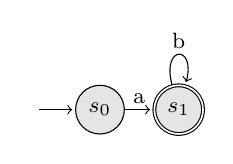
\begin{tikzpicture}[aut,node distance=1cm,font=\footnotesize]
  \node[st,initial]  (s_0)                 {$s_0$};
  \node[st,final]                    (s_2) [right of=s_0]  {$s_1$};
% 
  \path[->]
  (s_0) edge                node {a}  (s_2)
  (s_2) edge  [loop above]  node {b}  ();
\end{tikzpicture}}

\end{slide}


\begin{slide}{What are formal methods?}
  \centering

  \begin{minipage}{0.7\textwidth}
  \Large
  \begin{block}{}
    \centering
    Formal methods are \structure{techniques} to
    \\
    model \alert{complex systems} using
    \\
    \alert{rigorous mathematical models}

  \end{block}
  \end{minipage}
  \\[10mm]

  \begin{minipage}{0.32\textwidth}
  \begin{alertblock}{Specification}
    Define part of the system using a modelling language
  \end{alertblock}
  \end{minipage}
~~
  \begin{minipage}{0.3\textwidth}
  \begin{alertblock}{Verification}
    Prove properties.\\Show correctness.\\Find bugs.
  \end{alertblock}
  \end{minipage}
~~
  \begin{minipage}{0.28\textwidth}
  \begin{exampleblock}{Implementation}
    Generate correct code.\\
  \end{exampleblock}
  \end{minipage}

\end{slide}

\begin{frame}
  \huge\centering
  All formal models are \alert{wrong}
  \pause
  \\[5mm]
  ... but some of them are \structure{usefull}!
\end{frame}


% \begin{slide}{Many success cases}
%   \huge\centering

%   Cryptographic protocols
%   \\[5mm]
%   Distributed systems do not get stuck
%   \\[5mm]
%   Safety in railway systems
%   \\[5mm]
%   Type systems
%   \\[5mm]
%   \faded{\emph{[Tests: Validation (not Verification)]}}

% \end{slide}


\begin{slide}{Syllabus}
  \frsplitt{
  \begin{itemize}
    \item High-level overview or requirements and associated processes
    \\[5mm]
    \item Mathematical Preliminaries
    \begin{itemize}
      \item Basic mathematical notations
      \item Set theory
      \item PropositionalLogic
      % \begin{itemize}
      %   \item Syntax, semantics, and reasoning
      % \end{itemize}
      \item First Order Logic
      % \begin{itemize}
      %   \item Syntax, semantics, and reasoning
      % \end{itemize}
      \item The Z3 automatic theorem prover
      % \begin{itemize}
      %   \item Rise4fun interface: get acquainted with the tool
      %   \item Python API: automating search for solutions
      % \end{itemize}
    \end{itemize}
  \end{itemize}
  }{
  \begin{itemize}
    \alert{
    \item Behavioural modelling
    }
    \begin{itemize}
      \alert{
      \item Single component
      \begin{itemize}
        \item State diagrams and Flow charts
        \item Formal modelling: Automata, Process Algebra
      \end{itemize}
      \item Many components
      \begin{itemize}
        \item Communication diagrams and Sequence
  diagrams
        \item Formal modelling: Process algebra with interactions
      \end{itemize}
      }
      \item Equivalences
      % \begin{itemize}
      %   \item (Bi)similarity
      %   \item Realisability
      % \end{itemize}
      \item Verification
      % \begin{itemize}
      %   \item Verification of requirements
      %   \item Formal modelling: modal logics
      %   \item Tools: model checking with mCRL2
      % \end{itemize}
    \end{itemize}
  \end{itemize}
  }
\end{slide}


\section{UML behaviour diagrams}
%----------------------------------------------------------------------------------

\begin{slide}{UML behaviour diagrams}
  Describe the \structure{state} of a component, what \structure{actions} it can do, and how it \structure{evolves} during its life cycle.

  ~\\[5mm]

  \begin{itemize}
    \item \alert{State Diagram} focus on states
    \item \alert{Flowchart} focus on actions (also known as \emph{activity diagrams})
  \end{itemize}
\end{slide}


\begin{slide}{Coffee State Diagram}
  % \begin{block}{State Diagram}
    \includegraphics[width=1.0\textwidth]{images/diagrams/coffee-state.png}
  % \end{block}
\end{slide}

\begin{slide}{Coffee Flowchart}
  % \begin{block}{Flowchart}
    \includegraphics[width=1.0\textwidth]{images/diagrams/coffee-flow.png}
  % \end{block}
  \\[6mm]
  \frsplitt{
  \structure{Used symbols}: \emph{processes}, \emph{decisions}, and \emph{start/end}
  }{
  \structure{Other symbols} include: data (or input/output), documents, connectors, comments
  }
\end{slide}


\section{Automata -- Basic definitions}
%----------------------------------------------------------------------------------
\begin{slide}{Sequential and Reactive systems}
% \small

\frsplitt{\begin{block}{Sequential systems}
~\\[1mm]
Meaning is defined by the results of finite computations
\\[1mm]~
\end{block}}{
\begin{block}{Reactive systems}
~\\[1mm]
Meaning is determined by \structure{interaction} and \structure{mobility} of \structure{non-terminating} processes, 
evolving \structure{concurrently}
\\[1mm]~
\end{block}}

\bigskip

\frsplitt{\centering\alert{This module}}{\centering\alert{The next module}}


% \begin{block}{Reactive system}
% Meaning determined by \structure{interaction} and \structure{mobility} of \structure{non-terminating} processes, 
% evolving \structure{concurrently}
% \end{block}
% \caixa{system that computes by reacting to stimuli from its environment along its overall computation}
% \begin{itemize}
% \item in contrast to sequential systems whose meaning is defined by the results of finite computations, the behaviour of reactive systems is mainly determined by \structure{interaction} and \structure{mobility} of \structure{non-terminating} processes, 
% evolving \structure{concurrently}.
% \item \structure{observation} $\; \equiv\;$ interaction
% \item \structure{behaviour} $\; \equiv\;$ a structured record of interactions
% \end{itemize}
\end{slide}

%----------------------------------------------------------------------------------
\begin{slide}{Non-Deterministic Finite Automata (NFA)}
\small
\begin{block}{Definition}
A NFA over a set $\Act$ of names is a tuple
$\pair{S, I, \downarrow, \Act,  \rra}$ where
\begin{itemize}
\item $S = \enset{s_0, s_1, s_2, ...}$ is a set of \structure{states}
\item $I \subseteq S$ is the set of \structure{initial} states
\item  $\downarrow \subseteq S$ is the set of \structure{terminating} or final states
\begin{equation*}
\downarrow s \; \equiv\; s \in \downarrow
\end{equation*}
\item  $\rra \,\,\subseteq\, S \times \Act \times S$ is the \structure{transition} relation, often given as an $\Act$-indexed family of binary relations 
\begin{equation*}
s \rtran{a} s'\; \equiv\; \pair{s,a,s'} \in \rra
\end{equation*}
\end{itemize}
\end{block}
\end{slide}


\begin{slide}{Example}
  \begin{block}{Example of an automaton}
  \centering
  \wrap{
  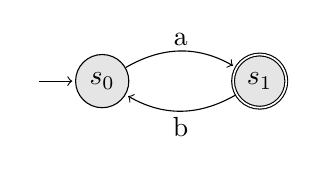
\begin{tikzpicture}[aut]
    \node[st,initial]  (s_0)                 {$s_0$};
    \node[st,final]  (s_1) [right of=s_0]  {$s_1$};
  % 
    \path[->]
    (s_0) edge[bend left] node {a}  (s_1)
    (s_1) edge[bend left] node {b}  (s_0);
  \end{tikzpicture}
  }
  ~~~~
  \wrap{$s_0$ is an initial state\\$s_1$ is a final state} 
  \end{block}
  %
  ~\\[-3mm]
  %
  \begin{block}{}
    \faded{(Formalise this automata)}
      \\[0.30\textheight]
  \end{block}

\end{slide}


\begin{slide}{Exercise}
\doExercise{Formalise these automata as $\pair{S,I,\dda,\Act,\rra}$}{
\centering
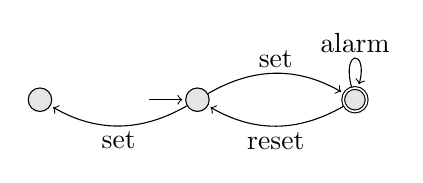
\begin{tikzpicture}[aut]
  \node[st] (s_0) {};
  \node[st,initial,right of=s_0] (s_1) {};
  % \node[st] (s_2) [right of=s_1]  {};
  \node[st,final] (s_2) [right of=s_1]  {};
% 
  \path[->]
  (s_1) edge[bend left] node {set} (s_2)
  (s_1) edge[bend left] node{set} (s_0)
  (s_2) edge  [loop above]  node {alarm} () edge[bend left] node{reset} (s_1);
\end{tikzpicture}
~~~~~~~~~~
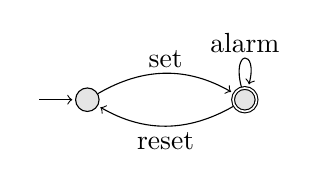
\begin{tikzpicture}[aut]
  \node[st,initial] (s_1) {};
  \node[st,final] (s_2) [right of=s_1]  {};
% 
  \path[->]
  (s_1) edge[bend left] node {set} (s_2)
  (s_2) edge  [loop above]  node {alarm} () edge[bend left] node{reset} (s_1);
\end{tikzpicture}

}
  
\end{slide}



    % \includegraphics[width=1.0\textwidth]{images/diagrams/coffee-state.png}

\begin{slide}{Exercise}
  \centering

  \vspace{-1mm}
  \includegraphics[width=1.0\textwidth]{images/diagrams/coffee-state.png}
  \vspace{-7mm}

  \doExercise{Draw LTS}{
      \faded{(suggestion: by hand on a paper, and take a photo of it.)}
      \\[0.20\textheight]
  }
\end{slide}


% \begin{slide}{Exercise}
%   \centering

%   \vspace*{-2mm}
%   \begin{columns}
%     \column{0.40\textwidth}\centering
%     \begin{block}{Flowchart}
%       \centering
%       \includegraphics[height=0.85\textheight]{images/cm-flowchart.png}
%     \end{block}
%     \column{0.56\textwidth}\centering
%     \doExercise{Draw LTS}{
%       \faded{(suggestion: by hand on a paper, and take a photo of it.)}
%       \\[0.75\textheight]
%     }
%   \end{columns}
% \end{slide}

%----------------------------------------------------------------------------------
% \begin{slide}{Labelled Transition System}
% \small
% \begin{block}{Morphism}
% A \structure{morphism} relating two LTS over  $\Act$, $\pair{S,\Act, \rra}$ and $\pair{S',\Act,  \rra'}$,
% is a function $\fdec{h}{S}{S'}$  st
% \begin{align*}
% s \rtran{a} s' \; \; \; \; \;  \imp & \; \; \; \; \; \apf{h}{s}  \primertran{a} \apf{h}{s'} 
% \end{align*}
% \end{block}

% \begin{center}
% \fbox{morphisms \structure{preserve} transitions}
% \end{center}
% \end{slide}

%----------------------------------------------------------------------------------
\begin{slide}{Labelled Transition System}
\small
% \begin{block}{System}
% Given an automaton $\pair{S, I, \dda, \Act, \rra}$, each state $s \in S$ determines a \structure{system} over 
% all states reachable from $s$ and the corresponding restriction of $\rra$.
% % and $\downarrow$.
% \end{block}

More generally, a NFA $\pair{S,I,\dda,\Act,\rra}$ is a \structure{labelled transition system} (LTS) $\pair{S,\Act,\rra}$, where each state $s \in S$ determines a \structure{system} over all states reachable from $s$ and the corresponding restriction of $\rra$.

\begin{block}{LTS classification}
\begin{itemize}
\item \alert{deterministic}
\item \alert{non deterministic}
\item \alert{finite}
\item \alert{finitely branching}
\item \alert{image finite}
\item ...
\end{itemize}
\end{block}

\end{slide}


%----------------------------------------------------------------------------------
% \begin{slide}{Language of an Automaton}
% \small

% Let $A = \pair{S, I, \dda, \Act,  \rra}$ be a NFA.

% \begin{block}{Transitive closure $\rra^{*}$}
% Let $N^{*}$ denote the set of all \structure{words} $a_1a_2\ldots a_n$, where $a_i \in N$ and $n \geq 0$. 
% The \alert{transitive closure} ${\rra^{*}} \subseteq S \times N^{*} \times S$, denoting $s\rtrant{w}s' \; \equiv\; (s,w,s') \in \rra^{*}$, be the minimal set satisfying:
% \begin{align*}
% \text{\alert{(1)}}\; \;  & 
%   s\in S \;\imp\; s \rtrant{\epsilon} s
%   % \rcb{\forall}{s}{s \in S}{s \rtrant{\epsilon} s}\\
% %
% \text{\alert{(2)}}\; \;  &
%   s \rtrant{w} s' \land s' \rtran{a} s'' \; \imp\;  s \rtrant{wa} s''
% %
% % \text{\alert{(2)}}\; \;  & 
%   % s \sigma \in \Tr{s}\; \imp\; \rcb{\exists}{s'}{s' \in S}{s \rtran{a} s'\, \e\, \sigma \in \Tr{s'}}
% \end{align*}


%----------------------------------------------------------------------------------
\begin{slide}{Reachability}
\small
\begin{block}{Definition}
The \structure{reachability relation}, ${\rra^*} \subseteq S \times \Act^* \times S$, is defined inductively
\begin{itemize}
\item $s \reach{\!\!\!\!\!\epsilon} s$ for each $s \in S$, where $\epsilon \in \Act^*$ denotes the empty \alert{word};
\item if  $s \rtran{a} s''$  and $s'' \reach{\!\!\!\!\!\sigma} s'$ then $s \reach{\!\!\!\!\!a \sigma} s'$, for $a \in \Act, \sigma \in \Act^*$
\end{itemize}
\end{block}

\begin{block}{Reachable state}
$t \in S$ is \structure{reachable} from $s \in S$ iff there is a \alert{word} $\sigma \in \Act^*$ st $s \reach{\!\!\!\!\!\sigma} t$
\end{block}

\end{slide}

\begin{slide}{Language of an Automaton}
\small

% Let $A = \pair{S, I, \dda, \Act,  \rra}$ be a NFA.

% \begin{block}{Transitive closure $\rra^{*}$}
% Define ${\rra^{*}} \subseteq S \times N^{*} \times S$ to be the \structure{transitive closure} of $\rra$ defined as the minimal set such that:
% \begin{align*}
% \text{\alert{(1)}}\; \;  & 
%   s\in S \;\imp\; (s,\epsilon,s) \in {\rra^{*}}\\  
% \text{\alert{(2)}}\; \;  &
%   (s,w,s') \in {\rra^{*}} ~\land~ s' \rtran{wa} s'' ~~\imp~~  (s,\epsilon,s'') \in {\rra^{*}}
% \end{align*}
% \end{block}

% Notation: $s\rtrant{w}s' \; \equiv\; (s,w,s') \in {\rra^{*}}$

\begin{block}{Language}
  \centering
  % The \structure{language $L_A$} of $A$ is the smallest set such that:
  % \begin{align*}
  %   s \in I ~\land~ s'\dda ~\land~ s\rtrant{w} s' ~~\imp~~ w \in L_A
  % \end{align*}
  A word $\sigma$ is in the \structure{language $L_A$} of an automata $A = \pair{S,I,\dda,N,\rra}$
  \\iff\\
  there are states $s\in I$, $s' \in \dda$ such that $s\rtrant{\sigma}s'$.
\end{block}
\end{slide}



\begin{slide}{Exercises}
\doExercise{What is the language of this automata?}{
\centering
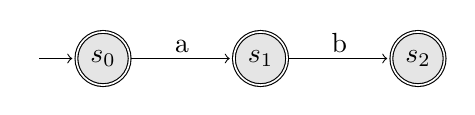
\begin{tikzpicture}[aut]
  \node[st,initial,final]  (s_0)                 {$s_0$};
  \node[st,final]                    (s_1) [right of=s_0]  {$s_1$};
  \node[st,final]                    (s_2) [right of=s_1]  {$s_2$};
% 
  \path[->]
  (s_0) edge                node {a}  (s_1)
  (s_1) edge                node {b}  (s_2);

\end{tikzpicture}
}

\doExercise{What is the language of this automata?}{
\centering
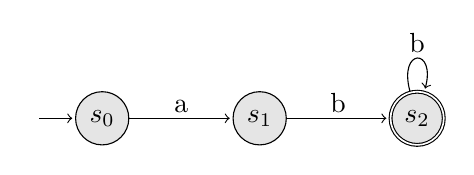
\begin{tikzpicture}[aut]
  \node[st,initial]  (s_0)                 {$s_0$};
  \node[st]                    (s_1) [right of=s_0]  {$s_1$};
  \node[st,final]                    (s_2) [right of=s_1]  {$s_2$};
% 
  \path[->]
  (s_0) edge                node {a}  (s_1)
  (s_1) edge                node {b}  (s_2)
  (s_2) edge  [loop above]  node {b}  ();
\end{tikzpicture}
}

\doExercise{What is the language of this automata?}{
\centering
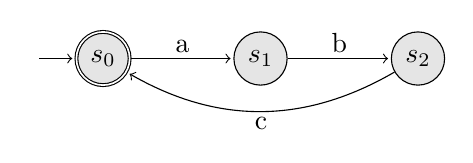
\begin{tikzpicture}[aut]
  \node[st,initial,final]  (s_0)                 {$s_0$};
  \node[st]                    (s_1) [right of=s_0]  {$s_1$};
  \node[st]                    (s_2) [right of=s_1]  {$s_2$};
% 
  \path[->]
  (s_0) edge                node {a}  (s_1)
  (s_1) edge                node {b}  (s_2)
  (s_2) edge[bend left] node {c}  (s_0);
\end{tikzpicture}
}

\end{slide}


\begin{slide}{Extra: Regular Expressions}

\begin{columns}[t]
  \colb[0.48]{Regular Expressions -- syntax}{
    \begin{itemize}
      \item \structure{$w_1w_2$}: word $w_1$ followed by word $w_2$
      \item \structure{$w_1+w_2$}: word $w_1$ or word $w_2$
      \item \structure{$a^{*}$}: 0 or more $a$'s
      \item \structure{$a^{+}$}: 1 or more $a$'s
      \item \structure{$\epsilon$}: empty word
    \end{itemize}
  }
  \col[0.48]{
    \begin{exampleblock}{Examples}
      \begin{itemize}
        \item \alert{$ab + c$}: ($a$ followed by $b$) or $c$
        \item \alert{$(ab)^{*}b$}: $b$ or $abb$ or $ababb$ or $\ldots$
        \item \alert{$c((ab)^{*}b)^{+}$}: $cb$ or $cabb$ or $cababb$ or $\ldots$
      \end{itemize}
    \end{exampleblock}
  }
\end{columns}

~\\\pause

\begin{block}{NFA vs. Reg. Expr.}
  \centering
  Word $w$ expressible by a NFA ~~$\Leftrightarrow$~~ $w$ expressible by a Reg. Expr.
\end{block}
  
\end{slide}


%----------------------------------------------------------------------------------
%\begin{slide}{An alternative characterisation}
%\small
%\begin{block}{Coalgebraic  characterization (morphism)}
%A \structure{morphism} $\fdec{h}{\pair{S, \nx}}{\pair{S', \nx'}}$ is a function 
%$\fdec{h}{S}{S'}$ st the following diagram commutes
%\begin{equation*}
%\xymatrix{
%S \times \Act \ar[d]_-{h \times \id} \ar[r]^-{\nx} & \ppow{S} \ar[d]^-{\ppow{h}}\\
%S' \times \Act \ar[r]^-{\nx'} & \ppow{S'}
%}
%\end{equation*}
%i.e.,
%\begin{equation*}
%\ppow{h} \comp \nx\; \; =\; \; \nx' \comp (h \times \id)
%\end{equation*}
%or, going pointwise,
%\begin{equation*}
%\setdef{\apf{h}{x}}{x \in \apf{\nx}{\pair{s,a}}}\; \;   =\; \;  \apf{\nx'}{\pair{\apf{h}{s},a}} 
%\end{equation*}
%\end{block}
%\end{slide}
%
%%----------------------------------------------------------------------------------
%\begin{slide}{An alternative characterisation}
%\small
%\begin{block}{Coalgebraic  characterization (morphism)}
%A \structure{morphism} $\fdec{h}{\pair{S, \nx}}{\pair{S', \nx'}}$ 
%\begin{itemize}
%\item \structure{preseves} transitions:
%\begin{equation*}
%s' \in \apf{\nx}{\pair{s,a}} \imp \apf{h}{s'} \in \apf{\nx'}{\pair{\apf{h}{s},a}} 
%\end{equation*}
%\item \structure{reflects} transitions:
%\begin{equation*}
%r' \in \apf{\nx'}{\pair{\apf{h}{s},a}} \imp \rcb{\exists}{s' \in S}{s' \in \apf{\nx}{\pair{s,a}}}{r' = \apf{h}{s'}}  
%\end{equation*}
%\end{itemize}
%\end{block}
%\alert{(why?)}
%\end{slide}
%
%
%%----------------------------------------------------------------------------------
%\begin{slide}{Comparison}
%\small
%
%\begin{itemize}
%\item Both definitions coincide at the \alert{object} level:
%\begin{equation*}
%\pair{s,a,s'} \in T\; \; \equiv\;\; s' \in \apf{\nx}{\pair{s,a}}
%\end{equation*}
%\item Wrt \alert{morphisms}, the relational definition is more general, corresponding, in coalgebraic terms to
%\begin{equation*}
%\ppow{h} \comp \nx\; \; \subseteq\; \; \nx' \comp (h \times \id)
%\end{equation*}
%\end{itemize}
%
%
%\pause
%
%%\begin{alertblock}
%\myblock{How can these notions of \structure{morphism} be used to compare LTS?}
%%\end{alertblock}
%
%
%\end{slide}


\section{Process algebra}

%-------------------------------------------------------------------------------
\begin{slide}{Process algebras}
\small

\begin{block}{Sequential CCS - Syntax}
\begin{equation*}
% \mathcal{P} ~\ni~ P,Q\; ::=\; K ~~|~~ \alpha.P ~~|~~ \sum_{i\in I} P_i
%         ~~|~~ \crn P f \faded{~~|~~ P|Q ~~|~~ P\backslash L}
\mathcal{P} ~\ni~ P,Q\; ::=\; K ~~|~~ \alpha.P ~~|~~ P + Q ~~|~~ \cnil
        ~~|~~ \crn P f  ~~|~~ P\backslash L \faded{~~|~~ P|Q}
\end{equation*}
%
where
\\- $\alpha \in \Act %\faded{\cup \overline\Act \cup \set{\tau}}
    \cup \set{\tau}$~ is an \structure{action}
\\- $K$ s a collection of \structure{process} names or process constants
\\- $I$ is an indexing set
\\- $L \subseteq \Act %\faded{\cup \overline{\Act}}
    $ is a set of \structure{labels}
\\- $f$ is a function that \structure{renames} actions s.t. $f(\tau) = \tau$ % and $f(\overline{a}) = \overline{f(a)}$
\\- \alert{notation:}
% \\~~~~~$\cnil = \sum_{i\in\emptyset}P_i$
% \\~~~~~$P_1+P_2 = \sum_{i\in\set{1,2}}P_i$
\\~~~~~$[f] = [a_1\mapsto b_1,\ldots,a_n \mapsto b_n]$
\end{block}
\end{slide}

%-------------------------------------------------------------------------------

\begin{slide}{Process algebras}
\small

\begin{block}{Syntax}
\begin{equation*}
% \mathcal{P} ~\ni~ P,Q\; ::=\; K ~~|~~ \alpha.P ~~|~~ \sum_{i\in I} P_i
%         ~~|~~ \crn P f \faded{~~|~~ P|Q ~~|~~ P\backslash L}
\mathcal{P} ~\ni~ P,Q\; ::=\; K ~~|~~ \alpha.P ~~|~~ P + Q ~~|~~ \cnil
        ~~|~~ \crn P f  ~~|~~ P\backslash L \faded{~~|~~ P|Q}
\end{equation*}
\end{block}

%\setcounter{equation}{0}
\begin{exampleblock}{\exercise Which are NOT syntactically correct? Why?}
\begin{columns}
  \column{0.38\textwidth}
  \begin{align}
    & a.b.A+B\\&
    (a.\cnil + b.A) \backslash \set{a,b,c}\\&
    (a.\cnil + b.A) \backslash \set{a,\tau}\\& % no
    a.B+[b\mapsto a]\\& % no
    \tau.\tau.B + \cnil
  \end{align}

  \column{0.45\textwidth}
  \begin{align} &
    a.(a + b).A\\&
    (a.B + b.B)[a\mapsto a,\tau\mapsto b]\\&
    (a.B + \tau.B)[b\mapsto a,a\mapsto a]\\& % no
    % (a.b.A + \ainv a.\cnil)|B\\&
    (a.b.A + b.\cnil).B\\&
    (a.b.A + b.\cnil)+B
    % \\&
    % (\cnil | \cnil) + \cnil
  \end{align}
\end{columns}
\end{exampleblock}

\end{slide}

%-------------------------------------------------------------------------------

\exerciseBack
\begin{slide}{CCS semantics - building a NFA}
\small 
\centering
\newcommand{\msep}{~~~~~~}

\typerule{act}{\shrk}{\alpha.P \trans\alpha P}
\msep
\typerule{sum-1}{P_1 \trans\alpha P'_1}{P_1 + P_2 \trans\alpha P'_1} %$\faded{j\in I}$
\msep
\typerule{sum-2}{P_2 \trans\alpha P'_2}{P_1 + P_2 \trans\alpha P'_2} %$\faded{j\in I}$
\\[3mm]
\typerule{res}{P\trans\alpha P'}{\crt P L\trans\alpha \crt{P'}L}~${\alpha%,\ainv{\alpha}
                                                                  \notin L}$
\msep
\typerule{rel}{P\trans\alpha P'}{\crn P f\trans{f(\alpha)} \crn{P'} f}
% \\[3mm]
% \typerule{com1}{P\trans\alpha P'}{P|Q\trans\alpha P'|Q}
% \msep
% \typerule{com2}{Q\trans\alpha Q'}{P|Q\trans\alpha P|Q'}
% \msep
% \typerule{com3}{P\trans a P' \quad Q\trans{\ainv{a}} Q'}{P|Q\trans\tau P'|Q'}
\\[6mm]

\only<1>{
  \begin{itemize}
    \item \structure{Initial states:} the process being translated
    \item \structure{Final states:} all states are final
    \item \alert{Language:} possible sequence of actions of a process
  \end{itemize}
}
\pause

\begin{exampleblock}{\exercise Build a derivation tree to prove the transitions below}
  % \vspace*{-4mm}
  \begin{enumerate}
    \item $(a.A + b.B) ~\trans{b}~ B$
    \item $(a.b.A + (b.a.B + c.a.C)) ~\trans{b}~ a.B$
    \item $((a.B + b.A)[a \mapsto c])\backslash\{a,b\} ~\trans{c}~ B$
  \end{enumerate}
\end{exampleblock}

\end{slide}

\begin{slide}{Exercise}
  \begin{exampleblock}{\exercise Draw the automata}
  % \vspace*{-4mm}
  \begin{align*}
    CM &= \mathsf{coin.coffee}.CM
    \\
    CS &= \mathsf{pub.(coin.coffee.CS + coin.tea.CS)}
    % CM &= \mathsf{coin.\ainv{coffee}}.CM
    % \\
    % CS &= \mathsf{\ainv{pub}.\ainv{coin}.coffee}.CS
    % \\
    % SmUni &= \crt{(CM|CS)}{\mathsf{\set{coin,coffee}}}
  \end{align*}
\end{exampleblock}

\doExercise{What is the language of this process?}{
\centering
  \vspace*{-5mm}
  \begin{align*}
    A &= \mathsf{goLeft.A + goRight.B}
    \\
    B &= \mathsf{rest.\cnil}
  \end{align*}
}
\end{slide}


\begin{slide}{Exercise}
  \centering

  \includegraphics[width=1.0\textwidth]{images/diagrams/coffee-flow.png}

  \doExercise{Write the process of the flowchart above}{
        $P ~~=~ \mf{powerOn} . Q$\\
        $Q ~~=~ \mf{selMocha}.\mf{addChocolate}.Mk + \mf{selLatte}.Mk + \ldots $\\
        $Mk ~=~ \mf{addMilk}\ldots$  
      ~\\[0.35\textheight]
  }

\end{slide}


% \begin{slide}{Exercise}
%   \centering

%   \vspace*{-2mm}
%   \begin{columns}
%     \column{0.40\textwidth}\centering
%     \begin{block}{Flowchart}
%       \centering
%       \includegraphics[height=0.85\textheight]{images/cm-flowchart.png}
%     \end{block}
%     \column{0.56\textwidth}\centering
%     \begin{exampleblock}{\exercise Write the processes}
%       \begin{align*}
%         P ~=~& \mf{powerOn} . Q\\
%         Q ~=~& \mf{selLatte}.L + \mf{selMocca}.M + \ldots \\
%         L ~=~& \ldots  
%       \end{align*}
%       ~\\[43mm]
%     \end{exampleblock}
%   \end{columns}
% \end{slide}
% %----------------------------------------------------------------------------------


\section{Concurrent Process algebra}

%-------------------------------------------------------------------------------
\begin{slide}{Process algebras}
\small

\begin{block}{CCS - \alert{Updated} Syntax}
\begin{equation*}
% \mathcal{P} ~\ni~ P,Q\; ::=\; K ~~|~~ \alpha.P ~~|~~ \sum_{i\in I} P_i
%         ~~|~~ \crn P f \transp{~~|~~ P|Q ~~|~~ P\backslash L}
\mathcal{P} ~\ni~ P,Q\; ::=\; K ~~|~~ \alpha.P ~~|~~ P + Q ~~|~~ \cnil
        ~~|~~ \crn P f  ~~|~~ P\backslash L ~~|~~ \alert{P|Q}
\end{equation*}
%
where
\\- $\alpha \in \Act \alert{\cup \overline\Act}
    \cup \set{\tau}$~ is an action
\\- $K$ s a collection of process names or process constants
\\- $I$ is an indexing set
\\- $L \subseteq \Act %\transp{\cup \overline{\Act}}
    $ is a set of labels
\\- $f$ is a function that renames actions s.t. $f(\tau) = \tau$  \alert{and $f(\overline{a}) = \overline{f(a)}$}
\\- notation:
% \\~~~~~$\cnil = \sum_{i\in\emptyset}P_i$
% \\~~~~~$P_1+P_2 = \sum_{i\in\set{1,2}}P_i$
\\~~~~~$[f] = [a_1\mapsto b_1,\ldots,a_n \mapsto b_n]$~~~~~where \alert{$a_i,b_i \in N \cup \set{\tau}$}
\end{block}
\end{slide}

%-------------------------------------------------------------------------------

\begin{slide}{Process algebras}
\small

\begin{block}{Syntax}
\begin{equation*}
% \mathcal{P} ~\ni~ P,Q\; ::=\; K ~~|~~ \alpha.P ~~|~~ \sum_{i\in I} P_i
%         ~~|~~ \crn P f \transp{~~|~~ P|Q ~~|~~ P\backslash L}
\mathcal{P} ~\ni~ P,Q\; ::=\; K ~~|~~ \alpha.P ~~|~~ P + Q ~~|~~ \cnil
        ~~|~~ \crn P f  ~~|~~ P\backslash L ~~|~~  \alert{P|Q}
\end{equation*}
\end{block}

%\setcounter{equation}{0}
\begin{exampleblock}{\exercise Which are syntactically correct?}
\begin{columns}
  \column{0.38\textwidth}
  \begin{align}
    & a.\ainv b.A+B\\&
    (a.\cnil + \ainv a.A) \backslash \set{\ainv{a},b}\\&
    (a.\cnil + \ainv a.A) \backslash \set{a,\tau}\\& % no
    (a.\cnil + \ainv{\tau}.A) \backslash \set{a}\\& % no
    % a.B+[b\mapsto a]\\& % no
    \tau.\tau.B + \ainv a.\cnil %\\&
    % a.(a + b).A
    \\&
    (\cnil | \cnil) + \cnil
  \end{align}

  \column{0.45\textwidth}
  \begin{align} &
    (a.B + b.B)[a\mapsto a,\tau\mapsto b]\\&
    (a.B + \tau.B)[b\mapsto a,b\mapsto a]\\& % no
    (a.B + b.B)[a\mapsto b,b\mapsto \ainv a]\\& % no
    (a.b.A + \ainv a.\cnil)|B\\&
    (a.b.A + \ainv a.\cnil).B\\&
    (a.b.A + \ainv a.\cnil)+B
  \end{align}
\end{columns}
\end{exampleblock}

\end{slide}

%-------------------------------------------------------------------------------

\begin{slide}{CCS semantics - building an NFA}
\small 
\centering
\newcommand{\msep}{~~~~~~}

\typerule{act}{\shrk}{\alpha.P \trans\alpha P}
\msep
\typerule{sum-1}{P_1 \trans\alpha P'_1}{P_1 + P_2 \trans\alpha P'_1} %$\transp{j\in I}$
\msep
\typerule{sum-2}{P_2 \trans\alpha P'_2}{P_1 + P_2 \trans\alpha P'_2} %$\transp{j\in I}$
\\[2mm]
\typerule{res}{P\trans\alpha P'}{\crt P L\trans\alpha \crt{P'}L}~$\transp{\alpha%,\ainv{\alpha}
                                                                  \notin L}$
\msep
\typerule{rel}{P\trans\alpha P'}{\crn P f\trans{f(\alpha)} \crn{P'} f}
\\[2mm]
\alert{
\typerule{com1}{P\trans\alpha P'}{P|Q\trans\alpha P'|Q}
\msep
\typerule{com2}{Q\trans\alpha Q'}{P|Q\trans\alpha P|Q'}
\msep
\typerule{com3}{P\trans a P' \quad Q\trans{\ainv{a}} Q'}{P|Q\trans\tau P'|Q'}
}
\\[5mm]
\pause

\begin{exampleblock}{\exercise Draw the NFAs}
  \exerciseBack
  \vspace*{-4mm}
  \begin{align*}
    % CM &= \mathsf{coin.coffee}.CM
    % \\
    % CS &= \mathsf{pub.(coin.coffee.CS + coin.tea.CS)}
    CM &= \mathsf{coin.\ainv{coffee}}.CM
    \\
    CS &= \mathsf{pub.\ainv{coin}.coffee}.CS
    \\
    SmUni &= \crt{(CM|CS)}{\mathsf{\set{coin,coffee}}}
  \end{align*}
  \vspace*{-7mm}
\end{exampleblock}
\end{slide}
\exerciseAdd



\begin{slide}{Exercises}
  \doExercise{Let $A=b.a.B$. Show that:}{
    \begin{enumerate}
      \item $(A ~|~ \overline{b}.\cnil)\backslash \{b\}\trans\tau (a.B ~|~ \cnil)\backslash\{b\}$
      \item $(A ~|~ b.a.B) + (b.A)[a/b] \trans{a} A[a/b]$
    \end{enumerate}
  }  
\end{slide}



%----------------------------------------------------------------------------------
\section{Sequence Diagrams vs. Interactive Processes}


%----------------------------------------------------------------------------------
\begin{slide}{Sequence Diagrams as Interactive Processes}
  \centering

  \includegraphics[width=0.6\textwidth]{images/sd-simple-atm.png}

  \frsplitdiff{0.57}{0.44}{
  \begin{itemize}
    \item \structure{Objects} as \alert{Processes}
    \\(e.g.,processes $U$, $A$, $C$, $B$)
    \item \alert{Send} actions (e.g., \mi{insertCard})
    \item \alert{Reveive} actions (e.g., \mi{\ainv{insertCard}})
    
  \end{itemize}
  }{\begin{itemize}
    \item Unique action for each object pair
    \item Do not write $(\ldots + \cnil)$
  \end{itemize}
  }
\end{slide}

%----------------------------------------------------------------------------------
\begin{slide}{Language of Sequence Diagrams, Informally}
  \centering

  \includegraphics[width=0.6\textwidth]{images/sd-simple-atm.png}

  \begin{exampleblock}{This example has only 1 word and its prefixes}
   $\Tr{sd} = \begin{array}[t]{l}
      insertCard \cdot verifyCard \cdot verifyAccount \cdot accountNotOK \cdot \\ rejectedCard \cdot ejectCard
      \end{array}$
  \end{exampleblock}
\end{slide}


%----------------------------------------------------------------------------------
\begin{slide}{Sequence Diagrams as Interactive Processes}
  \label{slide:sd as proc}
  \centering

  ~\\
  
  \begin{columns}
  \col[0.6]{
    \includegraphics[width=\textwidth]{images/sd-simple-atm.png}
  }
  \col[0.4]{
    \begin{exampleblock}{\exercise  Write an interactive processes that acts as above}
    $Sys = (U | A | C | E) \backslash \alert{\ldots}$
    \\~~$U = insertCard.\ainv{ejectCart}.\cnil$
    \\~~$A = \alert{\ldots}$
    \\~~$C = \alert{\ldots}$
    \\~~$E = \alert{\ldots}$
    \end{exampleblock}
  }
  \end{columns}
\end{slide}



%-------------------------------------------------------------------------------
% \section{Behavioural equivalences}

%----------------------------------------------------------------------------------

\end{document}

